% Template appropriated from another paper. May contain lots of legacy commands.

%\documentclass[times,10pt,twocolumn]{article} 
\documentclass[conference]{./IEEEtran}
%\documentclass{./IEEEtran}
\usepackage{amsmath, amsthm, amssymb, latexsym}
%\usepackage{latex8}
%\usepackage{times}

\usepackage[hyphens]{url}
\usepackage{pgfplots}
\usepackage{array}
\usepackage{multirow}
\usepackage{subfigure}
\usepackage{color}
\usepackage{framed}
\usepackage{graphicx}
\usepackage{tkz-graph}
\usepackage{bookmark}
%\usepackage[pdfstartview=FitH,colorlinks,linkcolor=blue,citecolor=blue]{hyperref}

\newcommand{\mysubsection}[1]{%
  \medskip
  \refstepcounter{subsection}%
    \everypar={%
      {\setbox0=\lastbox}% Remove the indentation
      \addcontentsline{toc}{subsection}{#1}%
      \textbf{{#1}.}
      \everypar={}%
    }%
  \ignorespaces
  % Dummy text in case there is no following text line (e.g. if the next thing is an itemize)
  %{\ }
  % TODO: MAKE SURE NO LINES ARE SWALLOWED BY THIS COMMAND.
}

\renewenvironment{leftbar}[1][\hsize]
{%
    \def\FrameCommand
    {%
        {\color{black}\vrule width 1pt}%
        \hspace{0pt}%must no space.
        \fboxsep=\FrameSep%
    }%
    \MakeFramed{\hsize#1\advance\hsize-\width\FrameRestore}%
}
{\endMakeFramed}


\newcommand{\algorithm}[2]{
%\begin{left bar}
\medskip
{\large \sc {#1}}
\medskip
\hrule
\smallskip
{#2}
\smallskip
\hrule
\medskip
%\end{leftbar}
}


\newcommand{\todo}[1]{\textcolor{red}{\textbf{[TODO: #1]}}}
\newcommand{\td}[2]{\textcolor{red}{\textbf{[TODO: {\it{#1}} #2]}}}


\newcommand{\site}[1]{\texttt{#1}}

\newcommand{\code}[1]{\texttt{#1}}
\newcommand{\quotedcode}[1]{{\vspace{0.5em}\normalfont{\code{#1}\vspace{0.5em}}}}


% Display all indices for development.
\newcommand{\draftonly}[1]{{\textcolor{orange}{#1}}}
%\renewcommand{\draftonly}[1]{}

% Theorem definitions
\theoremstyle{plain} 
\newtheorem{theorem}{Theorem}
\newtheorem{definition}{Definition} 

% For dev: page numbers with date.
\usepackage{fancyhdr}
\renewcommand{\headrulewidth}{0pt}
\fancyfoot[C]{Page \thepage\draftonly{\ -- Version: \today}}
\pagestyle{fancy}

\begin{document}


\title{The State of HSTS Deployment}

\author{}

% \author{
% Roy Frostig, Dan Boneh \\
% Stanford University \\
% \{rf,dabo\}@cs.stanford.edu \\
% \and
% Nicko van Someren \\
% Good Technology Inc. \\
% nicko@good.com
% }

\maketitle

% Page numbers on first page.
\thispagestyle{fancy}

\begin{abstract}

\end{abstract}

\section{Introduction}
\label{sec:intro}

\section{An Overview of HSTS}

\todo{short description}

There are three significantly distinct ways to send the HSTS header; these are describe clearly in 6797\todo{citation}:

\quotation{\it
The HSTS header field below stipulates that the HSTS Policy is to
remain in effect for one year (there are approximately 31536000
seconds in a year), and the policy applies only to the domain of the
HSTS Host issuing it:

\quotedcode{
Strict-Transport-Security: max-age=31536000
}

The HSTS header field below stipulates that the HSTS Policy is to
remain in effect for approximately six months and that the policy
applies to the domain of the issuing HSTS Host and all of its
subdomains:

\quotedcode{
Strict-Transport-Security: max-age=15768000 ; includeSubDomains
}

The HSTS header field below indicates that the UA must delete the
entire HSTS Policy associated with the HSTS Host that sent the header
field:

\quotedcode{
Strict-Transport-Security: max-age=0
}
}

\todo{Browser must only accept the HSTS header when it is sent over HTTPS}
\todo{Preload List}
\todo{The preload list overrides site settings in Chrome. See later for Firefox details.}

\section{Current Deployment by Top Sites}

Of the top 1000 sites in the Alexa rankings, $15$ are sending an HSTS header on a fresh request to their front page over HTTPS. The number of HSTS sites in the top $N$ grows roughly as ${1 \over 2}\sqrt{n}$. \todo{This includes sites sending a \code{max-age} of $0$, such as \site{facebook.com}.}

These numbers were found by using \code{curl} with a current Google Chrome user agent string \code{Mozilla/5.0 (Macintosh; Intel Mac OS X 10\_8\_5) AppleWebKit/537.36 (KHTML, like Gecko) Chrome/29.0.1547.76 Safari/537.36}. All results are from \todo{September 25, 2013}.

\begin{table}[htdp]
\label{alexa_table}
\begin{center}
\begin{tabular}{|r|c|l|}
\hline
$\#$ of top Alexa sites & \# HTTPS & \# HSTS\\
\hline
10 & 8 & 2 \\
\hline
100 & 64 & 4 \\	
\hline
1000 & 484 &15 \\
\hline
10000 & \todo{N/A} & 65\\
\hline
100000 & \todo{N/A} & \td{not final}{196}\\
\hline
\end{tabular}
\end{center}
\end{table}%

\begin{center}
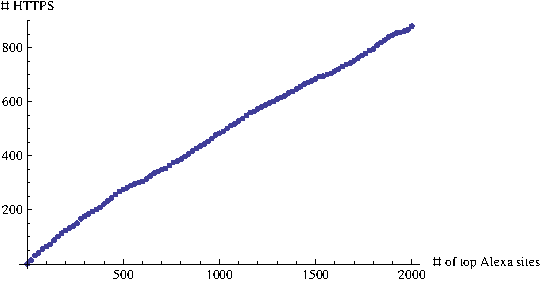
\includegraphics[width=70mm]{alexa_https.pdf}
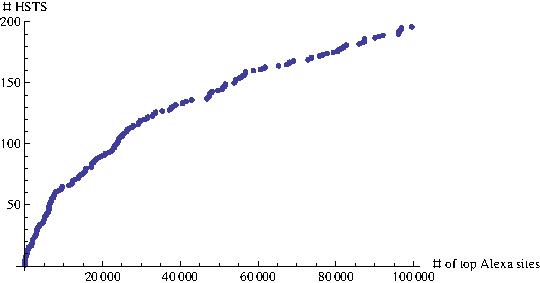
\includegraphics[width=70mm]{alexa_hsts.pdf}
\end{center}

\section{Common Deployment Patterns}

\section{Common Mistakes}

\section{Correct Practices}

\section{Browser Considerations}

\section{Conclusion}


\bibliographystyle{./IEEEtran}
\bibliography{paper}

\end{document}
